\subsection{Event Selection}
\label{sec:selection}

Initial event selection is outlined in Table~\ref{lab:eventsel}. This is primarily designed to remove problematic and background events in favour of the $Z\rightarrow\mu\mu + \text{jets}$ signal process. The various cuts are discussed in more detail below.

\begin{table}[h!]
    \centering
    \begin{tabular}{l|l}
         \hline
    \textbf{Event Selection} & \textbf{Description} \\ \hline
    Good Runs List & Event must be part of GRL \\ \hline
    Event Cleaning & No LAr, tile calorimeter, or tracker errors. Event is complete. \\ \hline
    Trigger & Single muon trigger: \\
    & HLT\_mu20\_iloose\_L1MU15\_OR\_HLT\_mu50 (2015) \\
    & HLT\_mu26\_ivarmedium\_OR\_HLT\_mu50 (2016-18) \\ \hline
    Primary Vertex & $N_{PV}\geq1$ \\ \hline
    Muons & $N_{\text{muons}}\geq2$ \\
          & Opposite charges \\
          & Pass TTVA recommendations for muons \\
          & $81\leq m_{\ell\ell} (\text{GeV})\leq 101$ \\
          & $p_{\text{T},\ell\ell}\geq200$ GeV \\ \hline
    \end{tabular}
    \caption{Overview of the applied event selection.}
    \label{lab:eventsel}
\end{table}

\subsubsection{Event Requirements}
The first requirement is that the event must be a part of the ATLAS Good Run Lists (GRL) [GRL Ref]. These are discussed in Sec.~\ref{sec:samples}.

Secondly, the events must pass event cleaning [Event Cleaning Ref]. This removes events that:
\begin{itemize}
    \item Contain errors in the data collected in the LAr calorimeters (check for error on xAOD::EventInfo::LAr)
    \item Contain errors in the data collected in the tile calorimeters (check for error on xAOD::EventInfo::Tile)
    \item Contain errors in the silicon tracker data (check for error on xAOD::EventInfo::SCT)
    \item Events which are incomplete due to a restart of the trigger, timing and control system (check for event flag in xAOD::EventInfo::Core)
    \item Events which fail the Loose event cleaning requirement (DFCommonJets\_eventClean\_LooseBad). This is also applied to MC samples.
\end{itemize}

Additionally, it is required that the event in question have at least one primary vertex.

\subsubsection{Trigger Requirements}
Events are required to pass an unprescaled single muon trigger, as outlined in Table~\ref{lab:eventsel} [Trigger Ref]. The recommended trigger is dependent on the year of the data (or corresponding Monte Carlo sample).

\subsubsection{Di-Muon System Requirements}
The event is required to have at least two muons of opposite charge, with a dilepton mass between 81 GeV and 101 GeV in order to ensure the muons originate from a $Z$ boson.

Additionally, the muons must pass track-to-vertex association recommendations [TTVA ref] as follows:

\begin{itemize}
    \item $|d_0^{BL}\text{significance}| < $ 3
    \item $|\Delta z_0^{BL}\sin\theta| < 0.5 $mm
\end{itemize}

where $d_0$ and $z_0$ represent the point along the track that is the closest approach to the beamspot.

The large $p_{\text{T},\ell\ell}$ cut of 200 GeV has been chosen to ensure that the balancing jet(s) have a high quantity of charged particles, as these are the primary subject of the analysis.

\subsection{Detector-level Objects}

\paragraph{Muons} are reconstructed using a combination of information from the muon spectrometer (MS) and the inner detector (ID). Occasionally, the ATLAS calorimeters are used to provide additional information for reconstruction. The reconstruction process is described in detail in reference [Muon Ref].
The muons are required to pass medium quality selection using the MuonSelectionTool and the PflowLoose\_VarRad isolation working point [Iso ref] as given by the IsolationTool. The simulated muons are also calibrated in order to correct for $p_\text{T}$ discrepancies between data and simulation [Muon Ref].

\paragraph{Tracks} are reconstructed from charged-particle hits within the silicon- and straw-tube based inner tracking detectors. They are required to pass the Loose quality working point and to be associated with the primary vertex of the event using the Tight track-to-vertex association.  The primary vertex is defined  as the reconstructed vertex with the highest sum of associated track $\pt^2$.  Tracks are required to have a $\pt>500$~\MeV~to be included in this measurement.  The track $\eta$ and $\phi$ coordinates come from the five-parameter track fit to $(\eta,\phi,q/p,d_0,z_0)$, and thus correspond to the track coordinates at the origin.

\paragraph{Jets} are reconstructed using the anti-$k_t$ algorithm [antikt Ref] with a radius parameter $R=0.4$. Particle flow objects [] are used as input. The jets are calibrated using the recommended procedure for small-R jets, this includes: MCJES calibration, global sequential calibration, and in-situ calibration.
Jets are required to have a calibrated $p_\text{T} > 10~\text{GeV}$ and rapidity $|y| < 4.4$.

\subsubsection{Overlap Removal}

There is a possibility that an electron may be misidentified as a jet during reconstruction, so in cases where the jet is found to be within $\Delta R < 0.2$ of a reconstructed electron, the jet is removed.
Additionally, a specialized overlap removal procedure must be applied between muons and jets due to a bug in the particle flow algorithm which results in secondary muon tracks being included in the particle flow objects.

A summary of the detector level event selection can be found in table~\ref{tab:ObjCuts}.


\begin{table}[h!]
    \centering
    \begin{tabular}{l|l}
    \hline
     \textbf{Object} & \textbf{Additional Selection Criteria} \\ \hline
     Calibrated Muons & Medium Quality, pass isolation: PflowLoose\_VarRad \\ \hline
     Calibrated Jets (AntiKt4EMPFlowJets) & $\Delta R_{e,jet} > 0.2$ \\
      & Muon-PFlow jet overlap removal \\ \hline
     Tracks & Loose Quality \\
      & Tight TTVA \\
      & $p_{\text{T}} > 500$ MeV \\ \hline
    \end{tabular}
    \caption{Object level cuts}
    \label{tab:ObjCuts}
\end{table}

\subsection{Particle-level Objects}

Stable charged particles ($c\tau$ > 10 mm) are used to define the analog of tracks at particle-level. Charged-particles are required to have $\pt > 500$~\MeV~and $|\eta|<2.5$.
Muons are dressed using all photons within a radius of $R=0.1$ and identical kinematic cuts are applied to those used at the detector-level.
TruthWZJets are utilized at the particle-level, which are constructed utilizing the anti-$k_t$ algorithm with $R=0.4$ from all particle 4-vectors except for prompt leptons from $W$, $Z$, Higgs, and $\tau$ decay, and photons within a cone of $R=0.1$ around the prompt lepton.
Objects at particle-level are summarized in table~\ref{tab:PLObjCuts}.

\begin{table}[h!]
    \centering
    \begin{tabular}{l|l}
    \hline
    \textbf{Object} & \textbf{Acceptance} \\ \hline
    Dressed Muons & $p_\text{T} \geq 25$ GeV, $|\eta| \leq 2.4$ \\\hline
    Jets (TruthWZJets) & $p_\text{T}\geq 10$ GeV, $|y|\leq4.4$ \\\hline
    Charged Hadrons & $p_\text{T} \geq 500$ MeV, $|\eta| \leq 2.5$  \\ \hline
    Phase Space & At least two oppositely charged muons \\
    & $81\leq m_{\ell\ell} \text{ (GeV)}\leq101$ \\
    & $p_{\text{T},\ell\ell}\geq200$ GeV \\ \hline
    \end{tabular}
    \caption{Fiducial object cuts}
    \label{tab:PLObjCuts}
\end{table}

\subsection{Corrections to Monte Carlo Samples}
\label{subsec:MCCorr}

\subsection{Data Stability Tests}
To check stability of data used for this analysis, rate for each year is calculated by dividing events to their corresponding luminosities. Luminosity per run is combined until summed up luminosities become either 2 fb$^{-1}$ or greater than this. Figure~\ref{fig:DataStability} depicts rate for year 2015 to 2018, where each time-ordered data bin contains 2 fb$^{-1}$ luminosity. The first bin shows rate for year 2015, bins 2--16 are for year 2016, bins 17--37 and 38--64 represent rate for year 2017 and 2018 respectively. Further, to consider those residual runs having combined luminosities smaller than 2 fb$^{-1}$, the last bin for each year is merged with the previous bin. The calculated average rate for year 2015--2018 is 2845 $\pm$ 4 and shows consistentency for each year. Figure~\ref{fig:DataStability} shows the stability of data for each year used in this analysis.
\begin{figure}[h!]
\centering
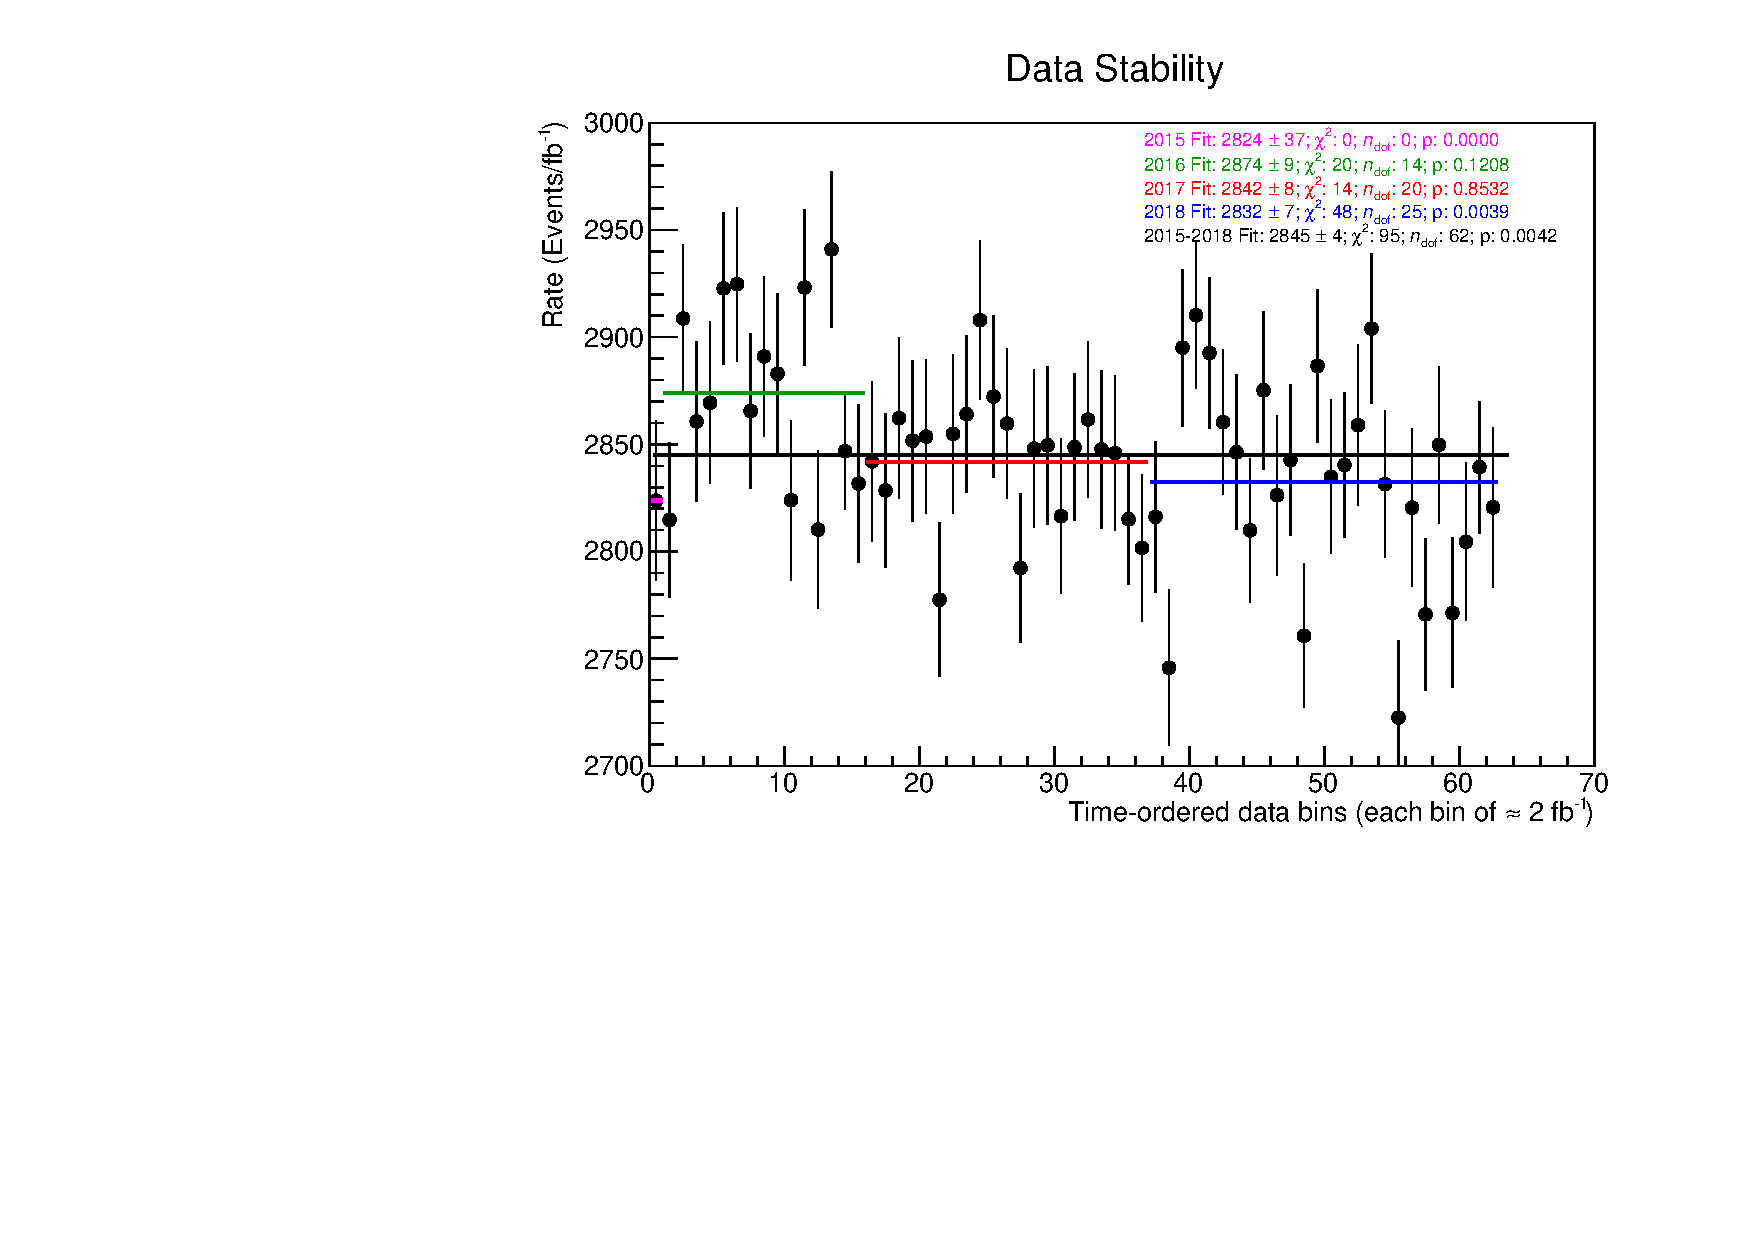
\includegraphics[width=0.75\textwidth]{figures/DataStability.pdf}
\caption{Events per fb$^{-1}$ for year 2015 to 2018, where each time-ordered data bin contains 2 fb$^{-1}$ luminosity.}
\label{fig:DataStability}
\end{figure}

\subsection{Data and Monte Carlo Comparison}
